% !TEX program = pdflatex
% Defensa TFM — Beamer (línea cronológica del documento)
\documentclass[aspectratio=169,11pt,professionalfonts]{beamer}

\usepackage[T1]{fontenc}
\usepackage{lmodern}
\usepackage[spanish]{babel}
\usepackage{amsmath,amssymb,bm}
\usepackage{booktabs}
\usepackage{tabularx}
\usepackage{graphicx}
\usepackage{tikz}
\usetikzlibrary{positioning,fit,arrows.meta,babel}
\usepackage[authoryear,round]{natbib}

\graphicspath{{../Imagenes/}{../../POCs/data/output/figures/}{../}}

% ── Theme ────────────────────────────────────────────────────────────
\usetheme{Madrid}
\usecolortheme{default}
\definecolor{unirazul}{RGB}{0,150,204}
\definecolor{ink}{RGB}{20,24,28}
\setbeamercolor{structure}{fg=unirazul}
\setbeamercolor{frametitle}{fg=ink,bg=white}
\setbeamercolor{title}{fg=ink}
\setbeamercolor{block title}{bg=unirazul,fg=white}
\setbeamercolor{block body}{bg=unirazul!6}
\setbeamerfont{frametitle}{series=\bfseries,size=\large}
\setbeamertemplate{navigation symbols}{}
\setbeamertemplate{footline}{%
  \hfill\insertframenumber/\inserttotalframenumber\hspace{1em}\vspace{4pt}%
}
\setbeamertemplate{itemize item}{\textcolor{unirazul}{$\bullet$}}
\setbeamertemplate{enumerate items}[default]

\title{Ventaja cuántica en ciencia de datos:\\
condiciones empíricas, métodos híbridos\\
y criterios de activación selectiva}
\subtitle{Defensa del Trabajo de Fin de Máster}
\author{Juan David Prada Malagón}
\institute{Máster en Computación Cuántica · UNIR\\[2pt]
Director: Ricardo Rafael Domínguez Reyes}
\date{}

\begin{document}

% =====================================================================
\section{Título}
% =====================================================================
\begin{frame}[plain]
  \titlepage
  \vspace{-1.2em}
  \begin{center}
    \footnotesize\textit{Documento:} \texttt{Documento/main.pdf} \quad
    \textit{Código:} \texttt{POCs/qml\_v2/}
  \end{center}
\end{frame}

\begin{frame}{Agenda (línea cronológica del TFM)}
\begin{columns}[T]
\begin{column}{0.48\textwidth}
\begin{enumerate}
  \item Motivación
  \item Introducción
  \item Contexto y estado de la técnica
  \item Planteamiento y metodología
  \item Resultados de modelos
\end{enumerate}
\end{column}
\begin{column}{0.48\textwidth}
\begin{enumerate}
  \setcounter{enumi}{5}
  \item Conjeturas ($\mathcal{Q}$, QCR)
  \item Análisis de las conjeturas
  \item Conclusiones
  \item Trabajo futuro
\end{enumerate}
\end{column}
\end{columns}
\vspace{0.8em}
\begin{block}{Estructura del documento}
Marco teórico (Cap.~1--3) $\rightarrow$ Implementación (Cap.~4--5) $\rightarrow$ Discusión y cierre (Cap.~6--8).
\end{block}
\end{frame}

% =====================================================================
\section{Motivación}
% =====================================================================
\begin{frame}{Motivación}
\begin{columns}[T]
\begin{column}{0.55\textwidth}
\begin{itemize}
  \item La ciencia de datos escala en dimensionalidad y complejidad combinatoria \citep{jordan2015, biamonte2017}.
  \item Los algoritmos variacionales y de kernel prometen ventaja en la era NISQ \citep{preskill2018, farhi2014, schuld2021}.
  \item Persiste una \textbf{brecha} entre promesas teóricas y evidencia reproducible sobre datos reales.
\end{itemize}
\end{column}
\begin{column}{0.42\textwidth}
\begin{block}{Pregunta práctica}
¿Cuándo activar un módulo cuántico\\
y cuándo quedarse con el stack clásico?
\end{block}
\end{column}
\end{columns}
\end{frame}

\begin{frame}{Estructura del TFM}
\centering
\begin{tikzpicture}[font=\scriptsize, thick, scale=0.85, every node/.style={transform shape},
    capnodo/.style={rectangle, rounded corners=4pt, very thick,
                minimum width=2.8cm, minimum height=0.75cm,
                align=center, inner sep=3pt},
    bloque/.style={rectangle, rounded corners=6pt, dashed,
                   inner sep=6pt, very thick},
    arr/.style={->, thick, gray!60}]
  \node[capnodo, draw=blue!55!black, fill=blue!8]  (c1) at (0,    0) {\textbf{Cap. 1}\\Introducción};
  \node[capnodo, draw=blue!55!black, fill=blue!8]  (c2) at (0,  -1.35) {\textbf{Cap. 2}\\Contexto};
  \node[capnodo, draw=blue!55!black, fill=blue!8]  (c3) at (0,  -2.7) {\textbf{Cap. 3}\\Objetivos};
  \node[capnodo, draw=orange!60!black, fill=orange!7] (c4) at (4.6, -1.35) {\textbf{Cap. 4}\\Metodología};
  \node[capnodo, draw=orange!60!black, fill=orange!7] (c5) at (4.6, -2.7) {\textbf{Cap. 5}\\Evaluación};
  \node[capnodo, draw=violet!60!black, fill=violet!7] (c6) at (9.2, -0.8) {\textbf{Cap. 6}\\QCR / $\mathcal{Q}$};
  \node[capnodo, draw=violet!60!black, fill=violet!7] (c7) at (9.2, -2.15) {\textbf{Cap. 7}\\Conclusiones};
  \node[capnodo, draw=violet!60!black, fill=violet!7] (c8) at (9.2, -3.5) {\textbf{Cap. 8}\\Futuro};
  \node[bloque, draw=blue!40,   fit=(c1)(c2)(c3),
        label={[blue!60!black, font=\scriptsize\bfseries]above:Marco teórico}]   {};
  \node[bloque, draw=orange!45, fit=(c4)(c5),
        label={[orange!65!black, font=\scriptsize\bfseries]above:Implementación}] {};
  \node[bloque, draw=violet!45, fit=(c6)(c7)(c8),
        label={[violet!60!black, font=\scriptsize\bfseries]above:Discusión y cierre}] {};
  \draw[arr] (c3.east)  -- ++(0.55, 0) |- (c4.west);
  \draw[arr] (c4.south) -- (c5.north);
  \draw[arr] (c5.east)  -- ++(0.55, 0) |- (c6.west);
  \draw[arr] (c6.south) -- (c7.north);
  \draw[arr] (c7.south) -- (c8.north);
  \draw[->, thick, dashed, gray!50]
    (c5.north east) to[out=25, in=200] node[midway, above, font=\tiny, gray!65]{valida} (c6.south west);
\end{tikzpicture}
\end{frame}

% =====================================================================
\section{Introducción}
% =====================================================================
\begin{frame}{Introducción --- planteamiento del problema}
El problema central del trabajo \citep{preskill2018, biamonte2017}:

\begin{quote}
\itshape
\textquestiondown{}En qué condiciones, y para qué tipos de problemas de ciencia de datos,
los algoritmos cuánticos disponibles en la era NISQ ofrecen una
ventaja real y medible frente a los algoritmos clásicos?
\end{quote}

\vspace{0.6em}
\begin{block}{Hipótesis operativa}
La ventaja es \textbf{real pero condicionada}:
\begin{enumerate}
  \item alineación \textbf{feature map} $\leftrightarrow$ \textbf{generador de datos}, o
  \item problema formulable como QUBO con arquitectura \textbf{híbrida} a escala viable.
\end{enumerate}
\end{block}
\end{frame}

\begin{frame}{Introducción --- alcance}
\begin{columns}[T]
\begin{column}{0.5\textwidth}
\textbf{Familias industriales (4)}
\begin{itemize}
  \item Clasificación supervisada (QSVM)
  \item Regresión (QK-SVR)
  \item Optimización combinatoria (QAOA)
  \item Optimización / híbrido (VQE + MDS)
\end{itemize}
{\footnotesize Extendidas a 9 protocolos justos en el documento (anomalías, TSP, lags,\ldots).}
\end{column}
\begin{column}{0.48\textwidth}
\textbf{Tres capas de datos}
\begin{enumerate}
  \item Sintéticos con estructura cuántica nativa \citep{liu2021}
  \item Práctica SKG Tecnología
  \item Referencia pública
\end{enumerate}
\end{column}
\end{columns}
\end{frame}

% =====================================================================
\section{Contexto y estado de la técnica}
% =====================================================================
\begin{frame}{Era NISQ}
\begin{block}{NISQ \citep{preskill2018}}
Dispositivos de escala intermedia \textbf{ruidosos}: qubits limitados, decoherencia, sin corrección de errores a gran escala.
\end{block}
\begin{itemize}
  \item Algoritmos viables hoy: \textbf{variacionales} (QAOA, VQE) e híbridos \citep{farhi2014, cerezo2021}.
  \item Kernels cuánticos: acceso a espacios de Hilbert de alta dimensión \citep{schuld2021, huang2021}.
  \item Distinción clave: \textbf{metodologías} maduras vs.\ \textbf{hardware} aún inmaduro.
\end{itemize}
\end{frame}

\begin{frame}{Comparaciones cuántico--clásico en la literatura}
\begin{itemize}
  \item Condiciones teóricas de ventaja de kernel: geometría de datos crítica \citep{huang2021}.
  \item Datasets donde el kernel cuántico es óptimo por construcción \citep{liu2021}.
  \item Concentración de kernels y límites prácticos \citep{thanasilp2022}.
  \item Gap empírico: pocos estudios \textbf{justos} sobre datos empresariales reales \citep{fastovets2019}.
\end{itemize}
\begin{alertblock}{Posicionamiento de este TFM}
Evidencia empírica + protocolos justos + diagnóstico $\mathcal{Q}(\mathcal{D})$ + QCR formalmente planteado.
\end{alertblock}
\end{frame}

% =====================================================================
\section{Planteamiento y metodología}
% =====================================================================
\begin{frame}{Metodología en cuatro fases}
\centering
\begin{tikzpicture}[font=\footnotesize,
    fase/.style={rectangle, rounded corners=4pt, very thick,
                 minimum width=11.2cm, minimum height=0.95cm,
                 align=center, inner sep=5pt},
    arr/.style={->, very thick, >=stealth}]
  \node[fase, draw=blue!60!black, fill=blue!9] (f1) {
    \textbf{Fase 1 --- Datos:} nativo / SKG / público $\cdot$ normalización $\cdot$ PCA};
  \node[fase, draw=orange!60!black, fill=orange!9, below=0.35cm of f1] (f2) {
    \textbf{Fase 2 --- Algoritmos:} QSVM $\cdot$ QK-SVR $\cdot$ QAOA $\cdot$ VQE vs.\ GB / RF / RBF};
  \node[fase, draw=teal!60!black, fill=teal!9, below=0.35cm of f2] (f3) {
    \textbf{Fase 3 --- Evaluación:} CV $\cdot$ Acc / F1 / $R^2$ / AUC $\cdot$ escalabilidad};
  \node[fase, draw=violet!60!black, fill=violet!9, below=0.35cm of f3] (f4) {
    \textbf{Fase 4 --- Híbrido:} integración QAOA--COBYLA $\cdot$ criterios de activación $\cdot$ QCR};
  \draw[arr] (f1)--(f2); \draw[arr] (f2)--(f3); \draw[arr] (f3)--(f4);
\end{tikzpicture}
\end{frame}

\begin{frame}{Formalismo --- kernel cuántico}
Mapa de características $\phi:\mathcal{X}\to\mathcal{H}$ (\texttt{ZZFeatureMap}) y kernel de fidelidad:
\begin{equation}
  \kappa(x_i,x_j)=\bigl|\langle\phi(x_i)\,|\,\phi(x_j)\rangle\bigr|^2
  \label{eq:fidelity_kernel}
\end{equation}
Clasificador: SVM / SVR / OCSVM sobre $K_{ij}=\kappa(x_i,x_j)$ frente a baseline RBF bajo el mismo protocolo \citep{schuld2021, liu2021}.

\vspace{0.4em}
\begin{block}{Principio de alineación}
La ventaja aparece cuando el \textbf{generador del dato} está alineado con el feature map.
ZZ es el mapa validado en este corpus; no el único admisible (Pauli, IQP,\ldots).
\end{block}
\end{frame}

\begin{frame}{Formalismo --- QAOA / VQE híbridos}
Problema combinatorio $\to$ QUBO $\to$ Hamiltoniano de Ising:
\begin{equation}
  \min_{x\in\{0,1\}^n} x^\top Q x
  \quad\Longrightarrow\quad
  H_C=\sum_{i} h_i Z_i + \sum_{i<j} J_{ij} Z_i Z_j
\end{equation}
Ansatz QAOA de profundidad $p$ \citep{farhi2014}:
\begin{equation}
  \lvert\psi(\bm\gamma,\bm\beta)\rangle
  = e^{-i\beta_p H_B}e^{-i\gamma_p H_C}\cdots e^{-i\beta_1 H_B}e^{-i\gamma_1 H_C}\lvert+\rangle^{\otimes n}
\end{equation}
Optimizador clásico (COBYLA) ajusta $(\bm\gamma,\bm\beta)$; el módulo cuántico propone candidatos.
\end{frame}

\begin{frame}{Diseño: 4 familias $\times$ 3 capas de datos}
\centering
\renewcommand{\arraystretch}{1.25}
\begin{tabular}{@{}lll@{}}
\toprule
\textbf{Familia} & \textbf{Cuántico} & \textbf{Clásico de referencia} \\
\midrule
Clasificación & QSVM (ZZ) & GB, RF, SVM-RBF \\
Regresión & QK-SVR & XGBoost, RF, SVR-RBF, Ridge \\
Optimización (asignación) & QAOA ($p{=}1$) & Greedy, búsqueda local, ILP \\
Portafolio / cobertura & VQE / QAOA-MDS & Markowitz, fuerza bruta \\
\bottomrule
\end{tabular}

\vspace{1em}
Cada familia se evalúa, cuando aplica, en:
\quad (i) \textbf{cuántico-nativo}, \quad (ii) \textbf{SKG}, \quad (iii) \textbf{referencia pública}.
\end{frame}

% =====================================================================
\section{Resultados de modelos}
% =====================================================================
\begin{frame}{Resultados --- principio de alineación}
\begin{columns}[c]
\begin{column}{0.48\textwidth}
\centering
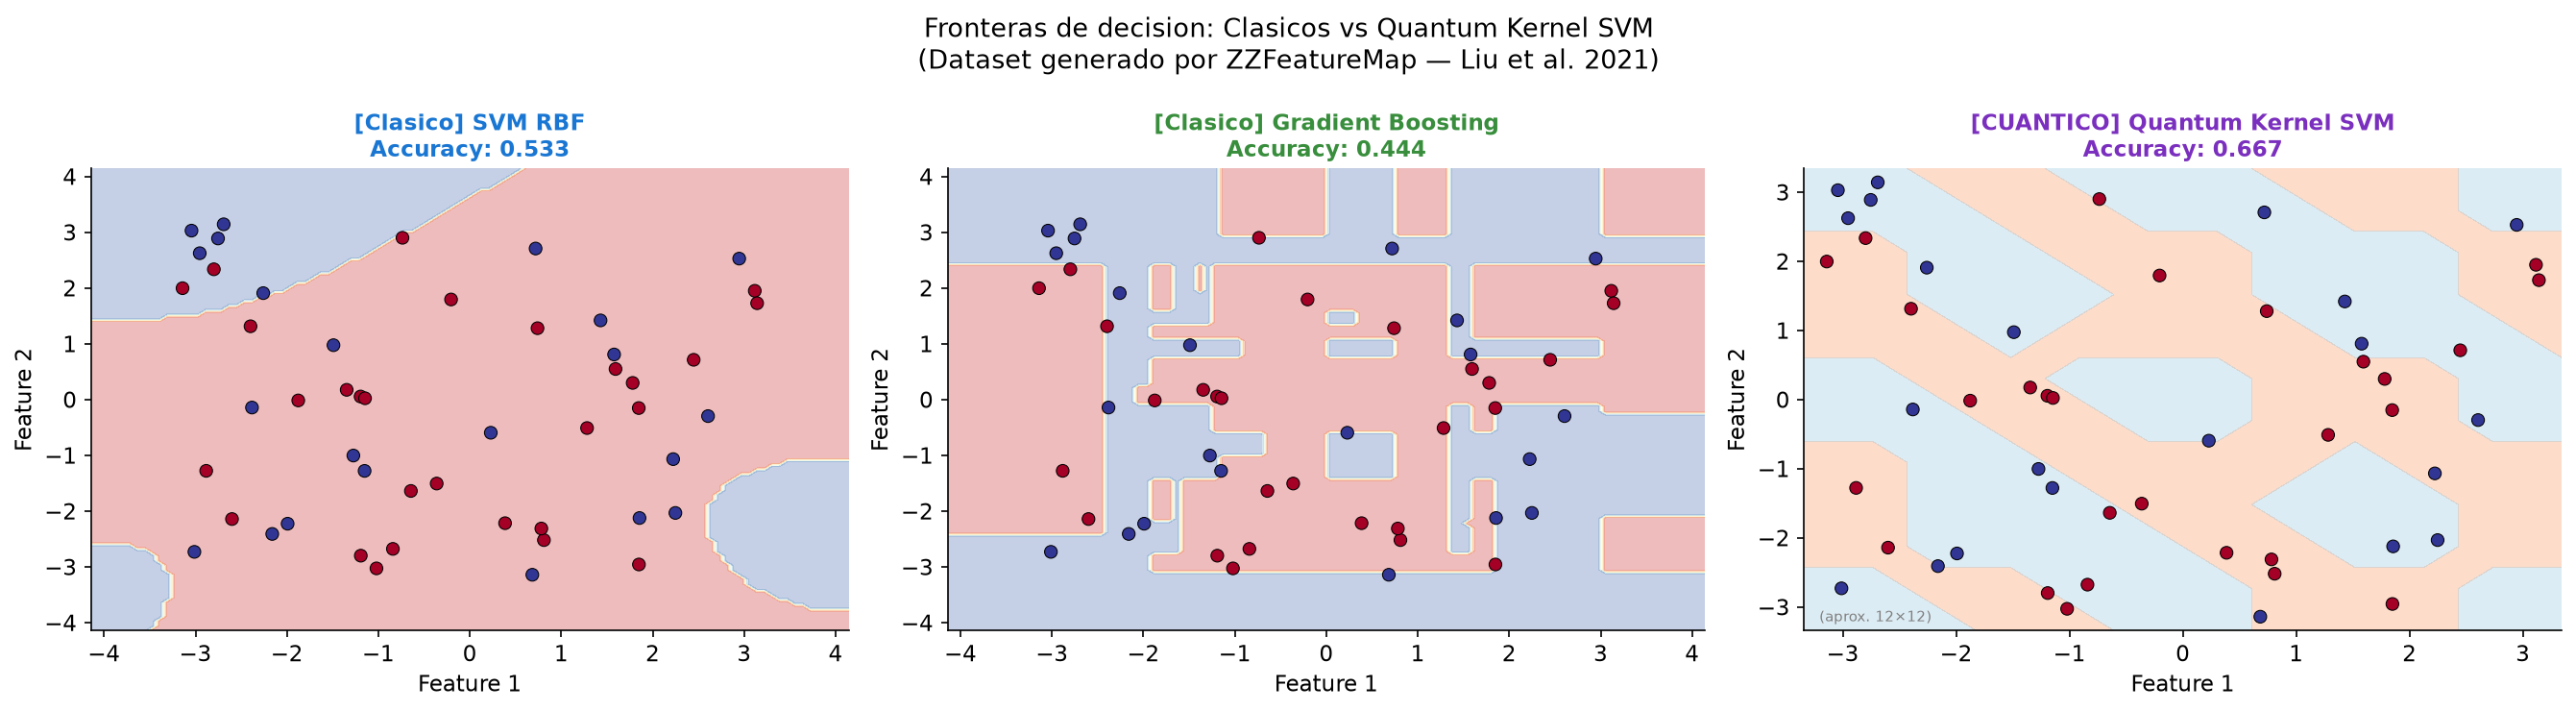
\includegraphics[width=\textwidth]{06_quantum_kernel_boundaries.png}
\end{column}
\begin{column}{0.48\textwidth}
\centering
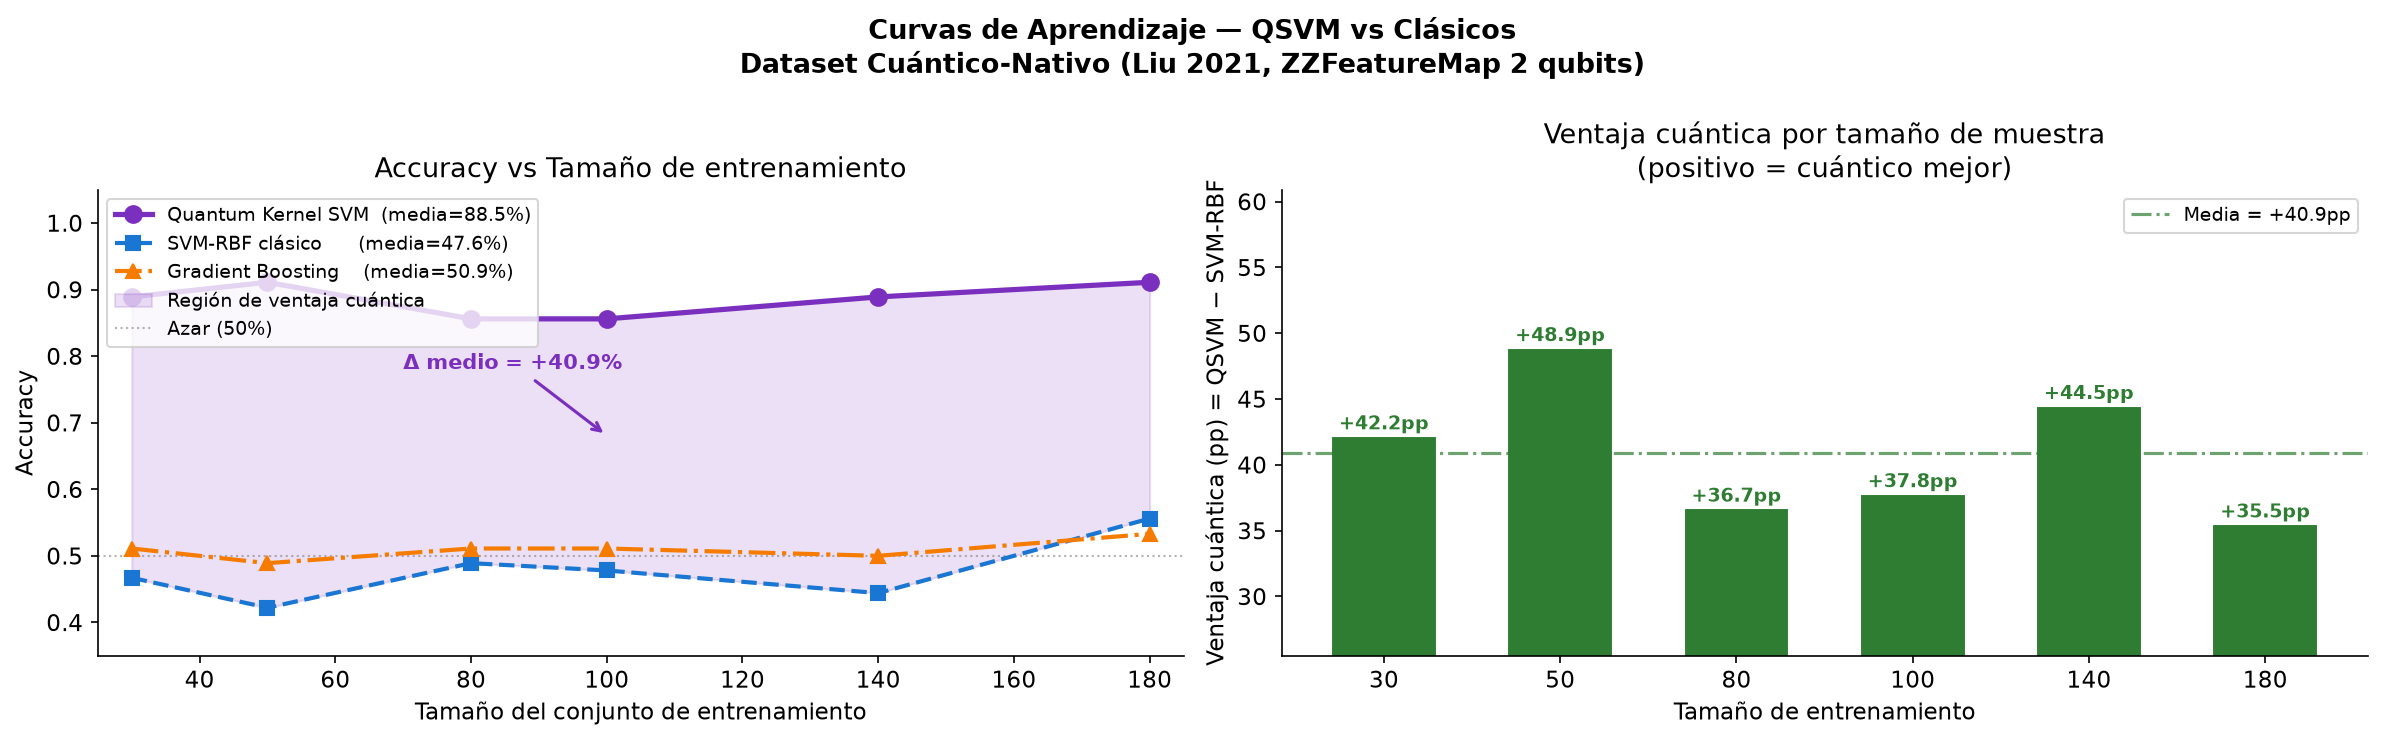
\includegraphics[width=\textwidth]{06_learning_curves_quantum_advantage.png}
\end{column}
\end{columns}
\end{frame}

\begin{frame}{Resultados --- clasificación}
\begin{columns}[T]
\begin{column}{0.62\textwidth}
\centering
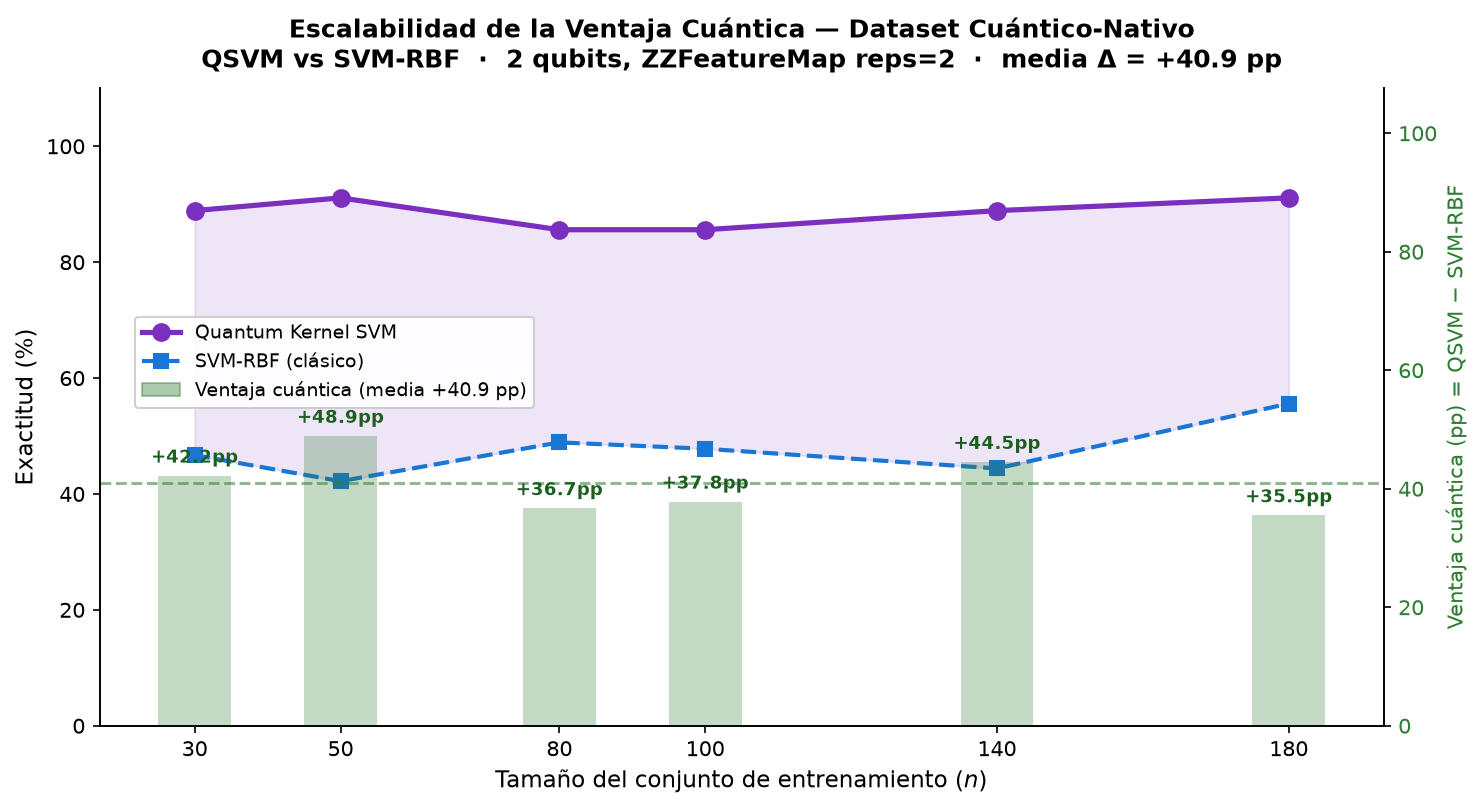
\includegraphics[height=0.72\textheight]{01_escalabilidad_ventaja_clasificacion.png}
\end{column}
\begin{column}{0.35\textwidth}
\begin{block}{Cifras ancla}
\begin{itemize}
  \item \textbf{+38.3\,pp} en datos alineados al mapa
  \item Media \textbf{+40.9\,pp} ($n\in[30,180]$)
  \item En Telco/SKG \textbf{sin} alineación: gana el clásico
\end{itemize}
\end{block}
\end{column}
\end{columns}
\end{frame}

\begin{frame}{Resultados --- optimización híbrida}
\begin{columns}[T]
\begin{column}{0.58\textwidth}
\centering
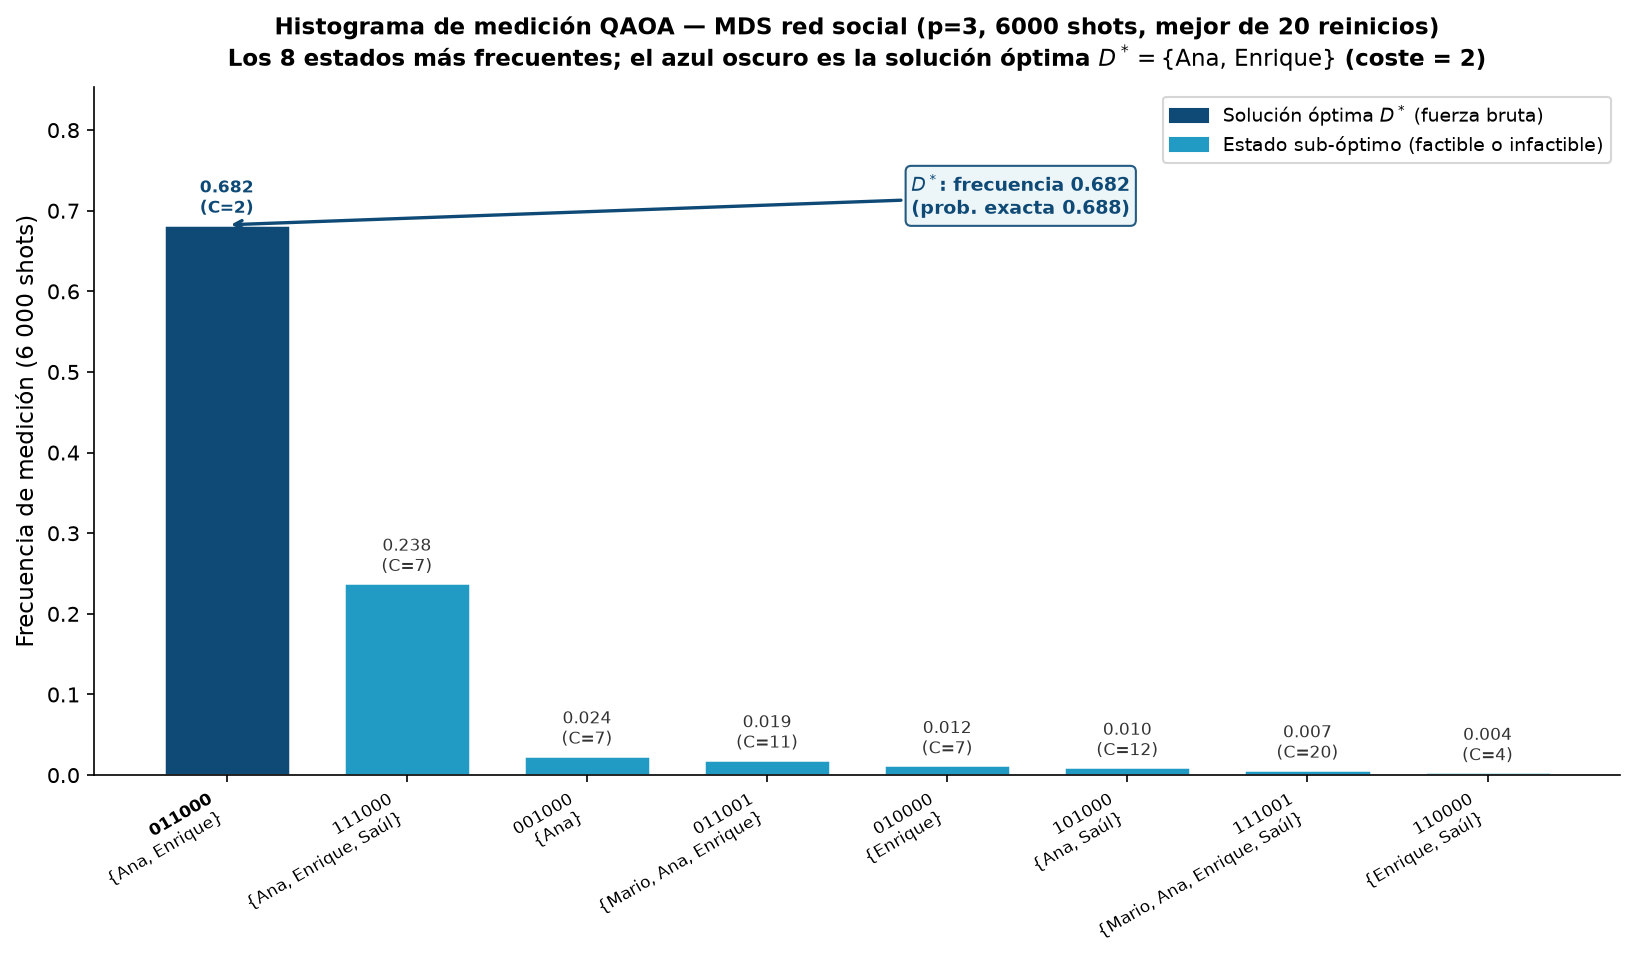
\includegraphics[height=0.68\textheight]{10_qaoa_histograma_medicion.png}
\end{column}
\begin{column}{0.40\textwidth}
\begin{block}{Hallazgos}
\begin{itemize}
  \item QAOA: \textbf{$-$30.3\%} coste vs.\ Greedy
  \item VQE competitivo en portafolio pequeño
  \item MDS: $P(\mathrm{opt})\approx 73\%$ (patrón híbrido)
  \item TSP $n{=}4$: empate óptimo --- valor de \emph{modelado}, no speedup
\end{itemize}
\end{block}
\end{column}
\end{columns}
\end{frame}

\begin{frame}{Síntesis visual de ventaja}
\centering
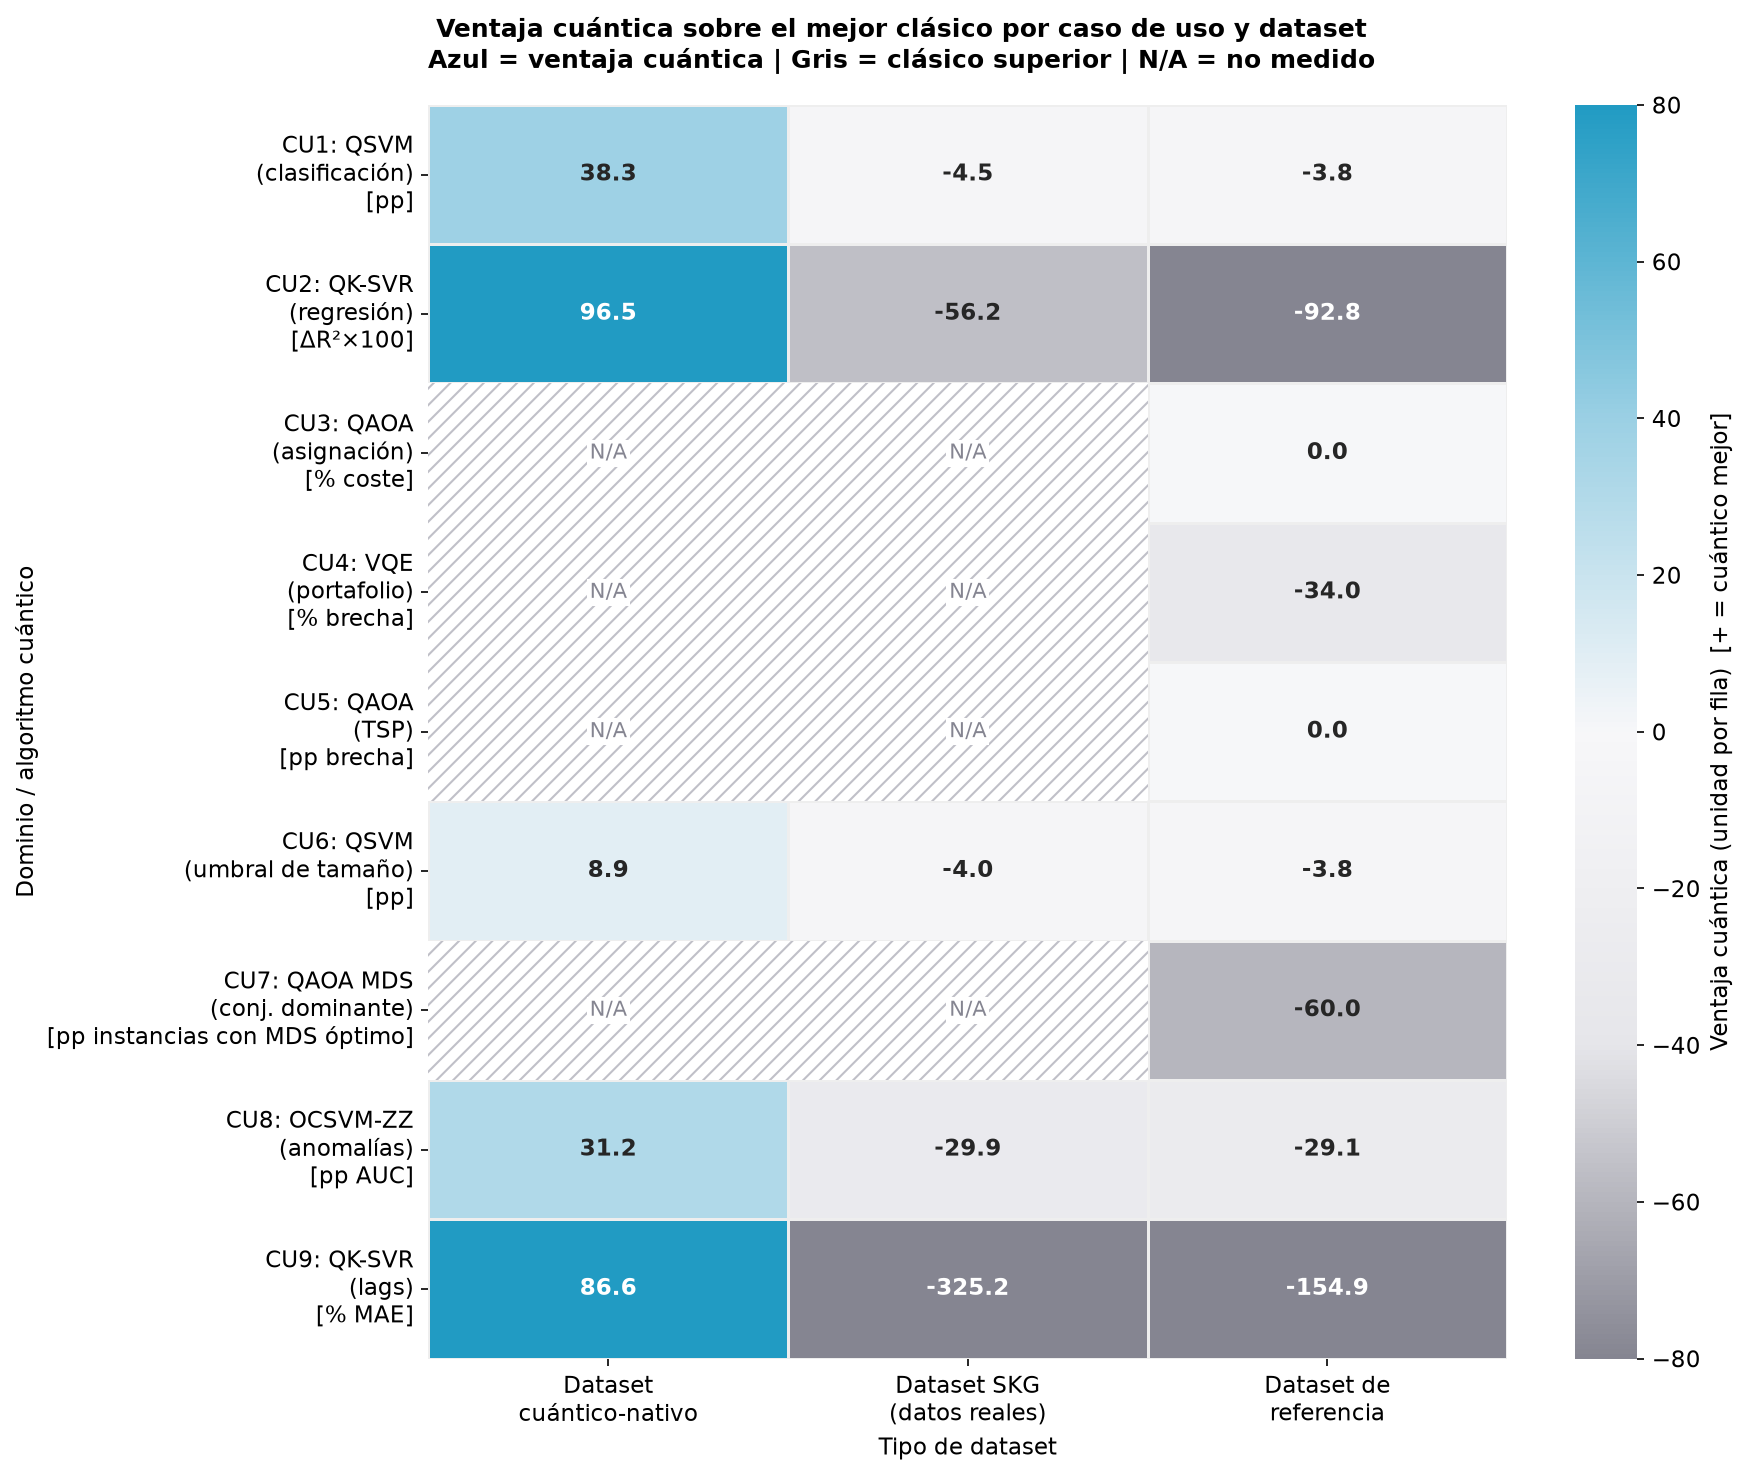
\includegraphics[height=0.78\textheight]{07_heatmap_ventaja_por_dominio.png}
\end{frame}

% =====================================================================
\section{Conjeturas}
% =====================================================================
\begin{frame}{De la evidencia a las preguntas originales}
Tras observar ventaja \textbf{solo} con alineación mapa--generador:

\begin{enumerate}
  \item \textbf{Tests de cuanticidad:}
  \textquestiondown{}Existe algún indicador calculable \emph{a priori} sobre un dataset que permita
  predecir si un algoritmo cuántico mostrará ventaja sobre los clásicos?

  \item \textbf{Mapeos cuántico-compatibles:}
  Si un dataset no tiene estructura cuántica nativa, \textquestiondown{}puede transformarse
  a un espacio de representación donde la tenga, sin alterar la información discriminativa?
\end{enumerate}
\end{frame}

\begin{frame}{Conjetura 1 --- score de cuanticidad $\mathcal{Q}(\mathcal{D})$}
\begin{equation}
  \mathcal{Q}(\mathcal{D})=w_1\Delta A + w_2\hat{d}_F + w_3\Delta H,
  \qquad \sum_i w_i=1,\; w_i\ge 0
  \label{eq:Q}
\end{equation}
donde
\begin{align*}
  \Delta A &= A(K_Q,K_y)-A(K_{\mathrm{RBF}},K_y),\\
  \hat{d}_F &= \|K_Q-K_{\mathrm{cl}}^\star\|_F\big/d_{F,\max},\\
  \Delta H &= H(K_Q)-H(K_{\mathrm{RBF}}).
\end{align*}
\begin{block}{Interpretación}
$\mathcal{Q}(\mathcal{D})>0$ predice ventaja estructural del kernel cuántico;
$\mathcal{Q}(\mathcal{D})<0$ predice superioridad clásica.
Coherente con la geometría de \citet{huang2021}.
\end{block}
\end{frame}

\begin{frame}{Conjetura 2 --- espacio de representación QCR}
Si $\mathcal{Q}(\mathcal{D})\le 0$, la conjetura afirma existencia de $\mathcal{Z}$ y $\psi:\mathcal{X}\to\mathcal{Z}$ \textbf{polinómica} tales que
\begin{equation}
  \mathbf{x}\xrightarrow{\psi}\mathbf{z}\xrightarrow{f_Q^\star}\hat{y}
  \qquad\text{con}\quad
  \mathcal{Q}(\psi(\mathcal{D}))>0
  \;\;\text{y}\;\;
  \varepsilon(f_Q^\star\circ\psi)\le\varepsilon(f_C^\star).
\end{equation}
\begin{alertblock}{Estado}
Conjetura \textbf{abierta}. Este TFM la \textbf{plantea formalmente} y aporta evidencia preliminar --- no una demostración.
\end{alertblock}
\end{frame}

% =====================================================================
\section{Análisis de las conjeturas}
% =====================================================================
\begin{frame}{Análisis P1 --- tests de cuanticidad}
\begin{columns}[c]
\begin{column}{0.48\textwidth}
\centering
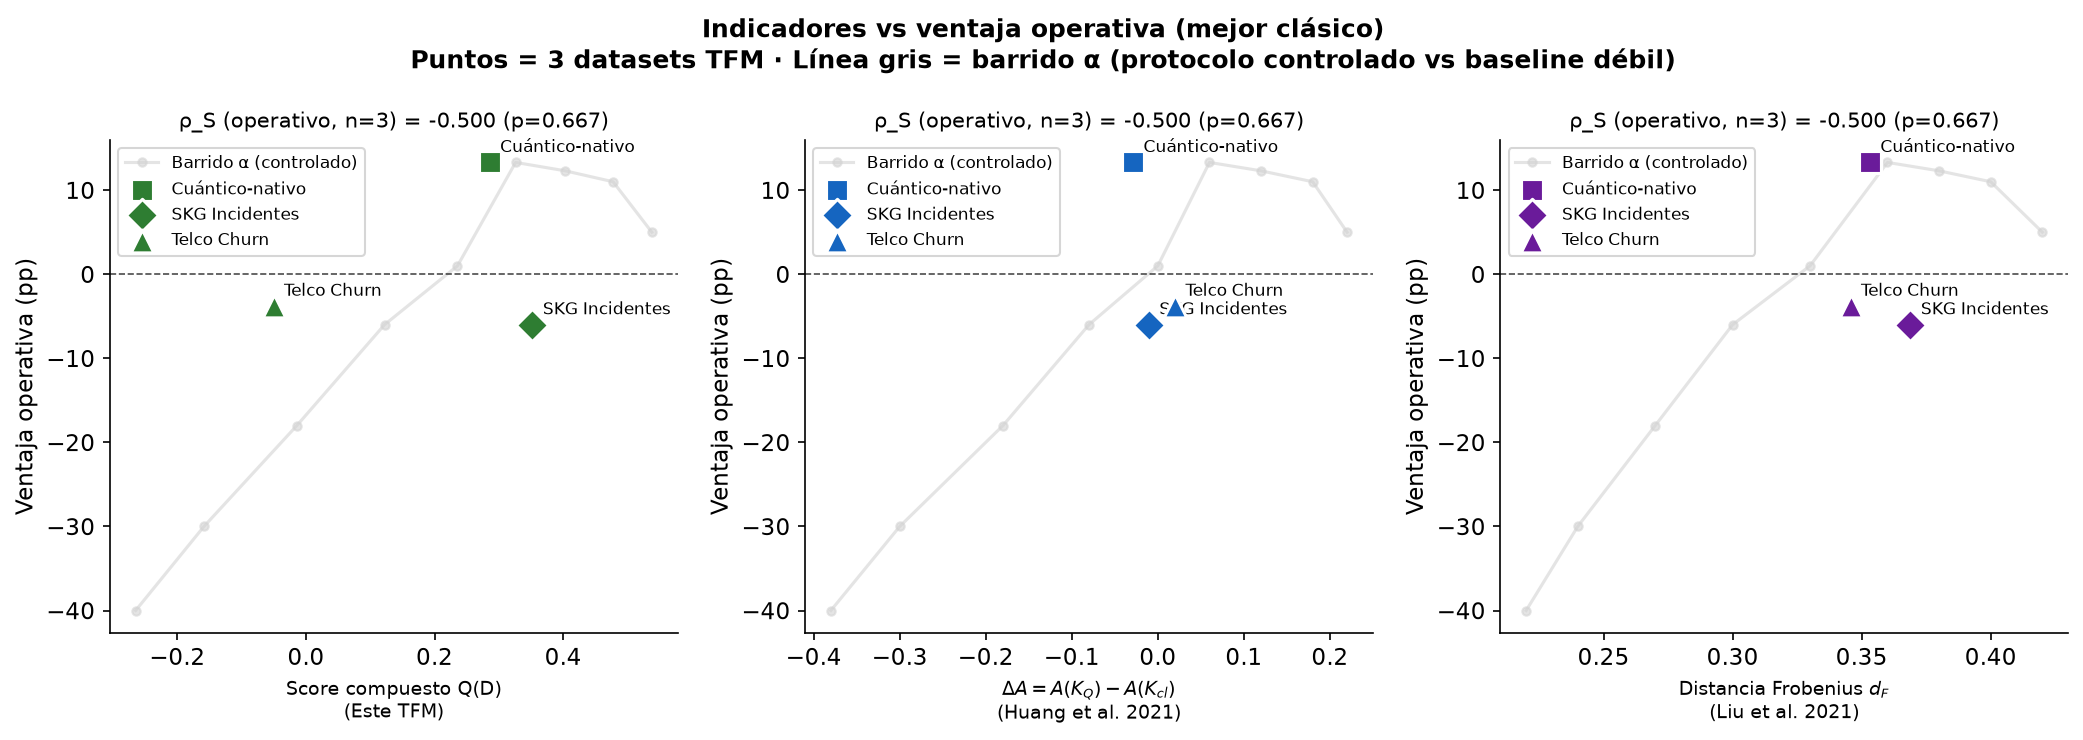
\includegraphics[width=\textwidth]{08_correlacion_indicadores_ventaja.png}
\end{column}
\begin{column}{0.48\textwidth}
\centering
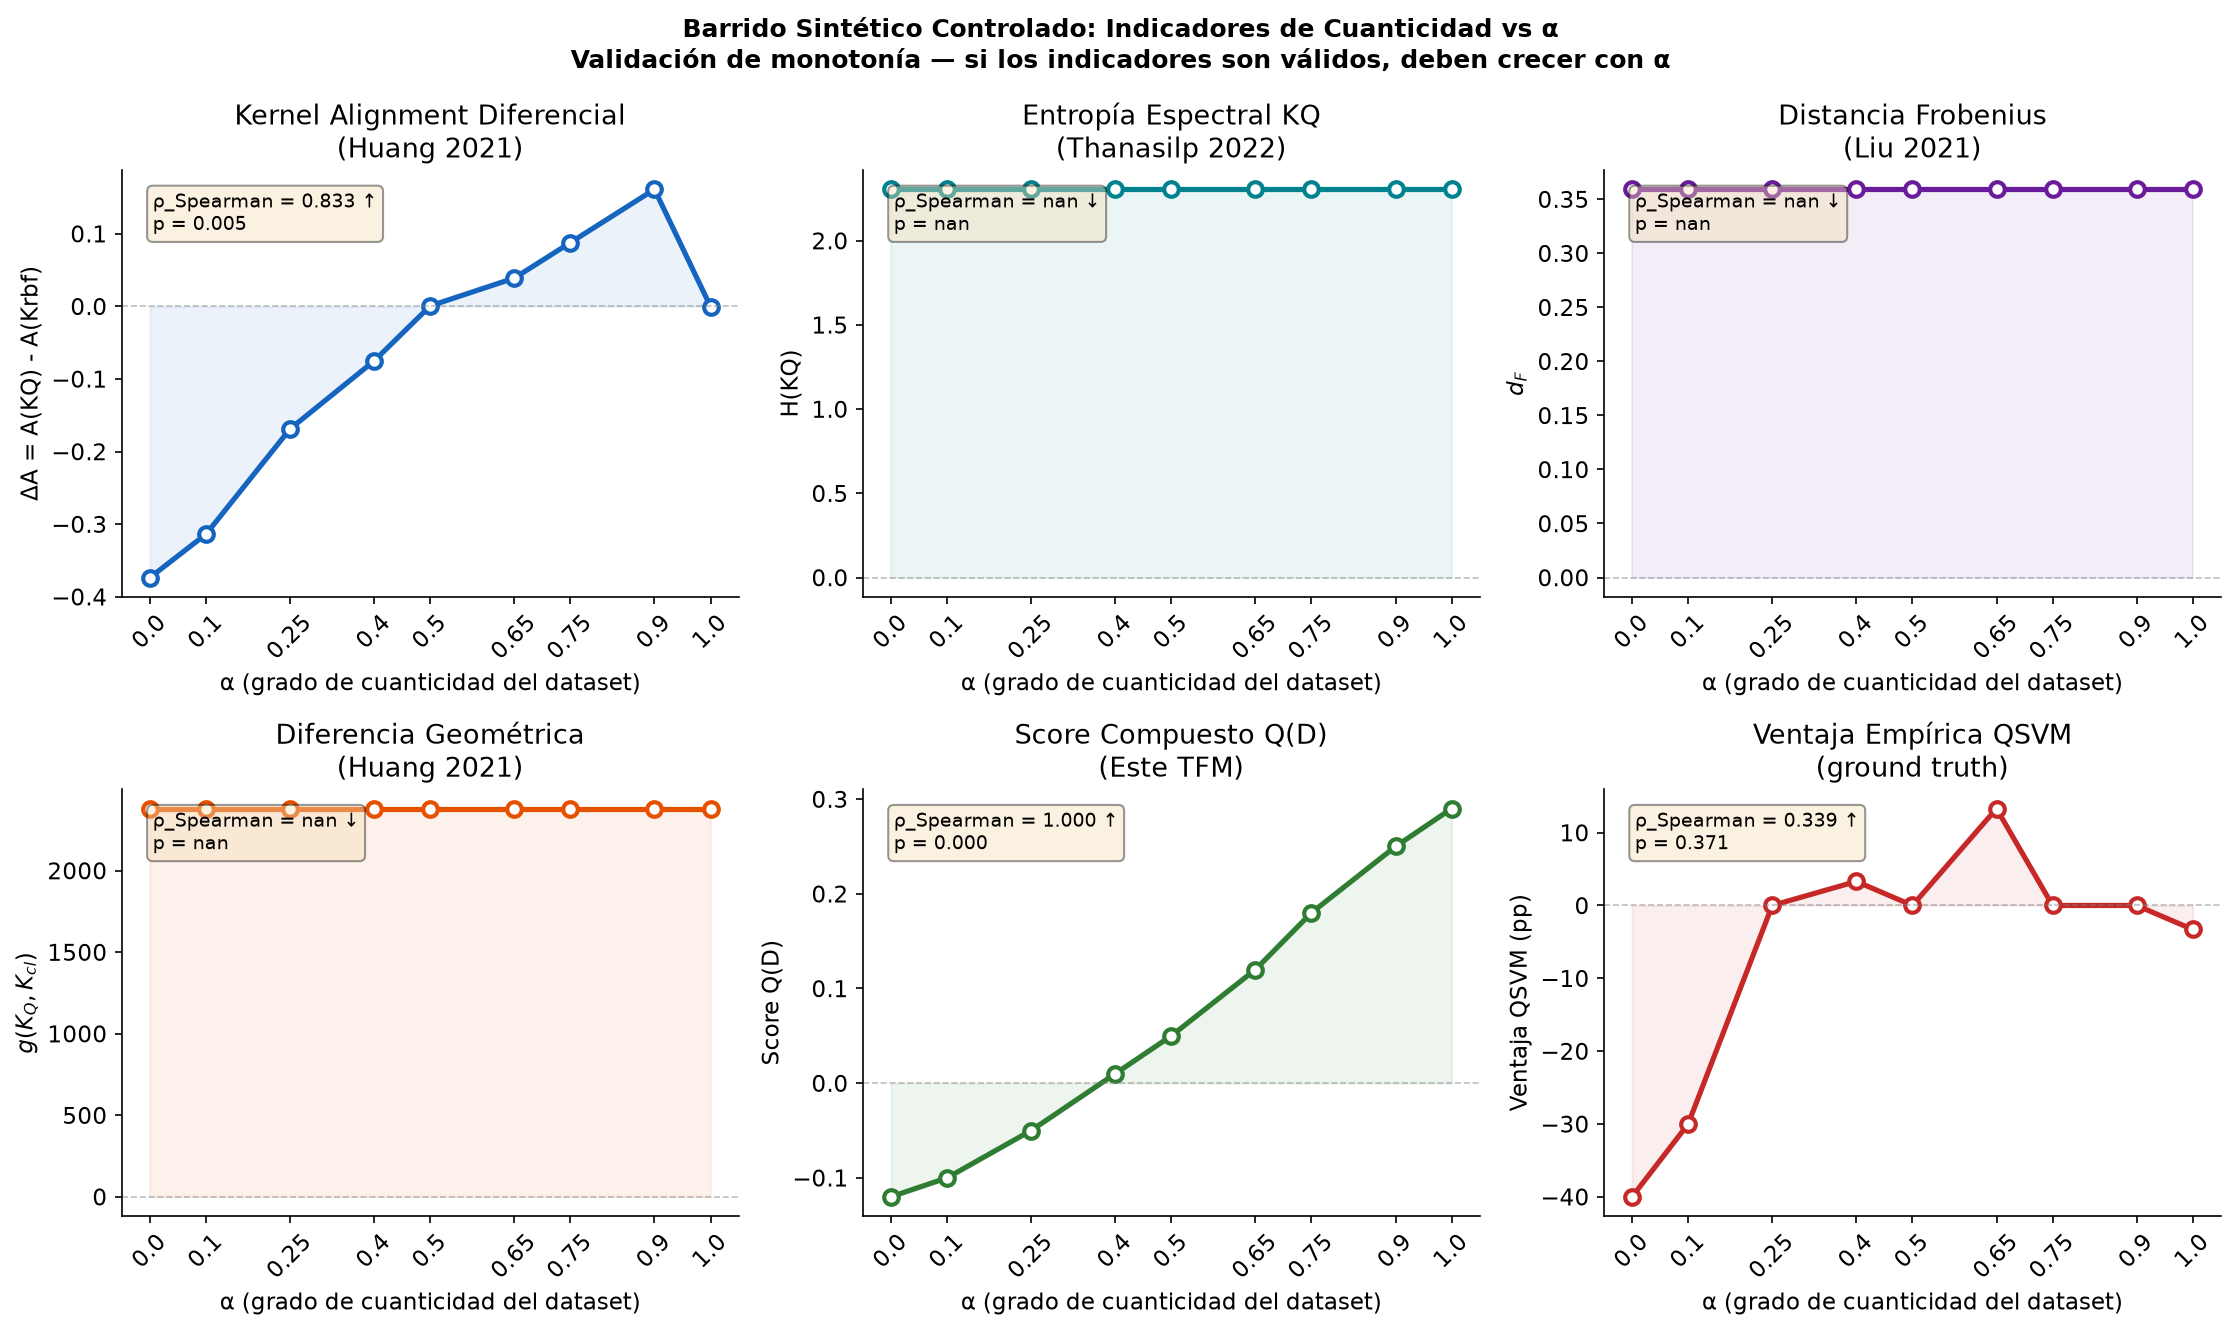
\includegraphics[width=\textwidth]{08_barrido_sintetico_alpha.png}
\end{column}
\end{columns}
\vspace{0.3em}
\centering\footnotesize
Barrido sintético: $\rho_S(\mathcal{Q},\mathrm{ventaja})=0.833$ ($p=0.005$, $n=9$). Componente más informativo: $d_F$.
\end{frame}

\begin{frame}{Análisis P2 --- mapeos cuántico-compatibles}
\begin{columns}[c]
\begin{column}{0.48\textwidth}
\centering
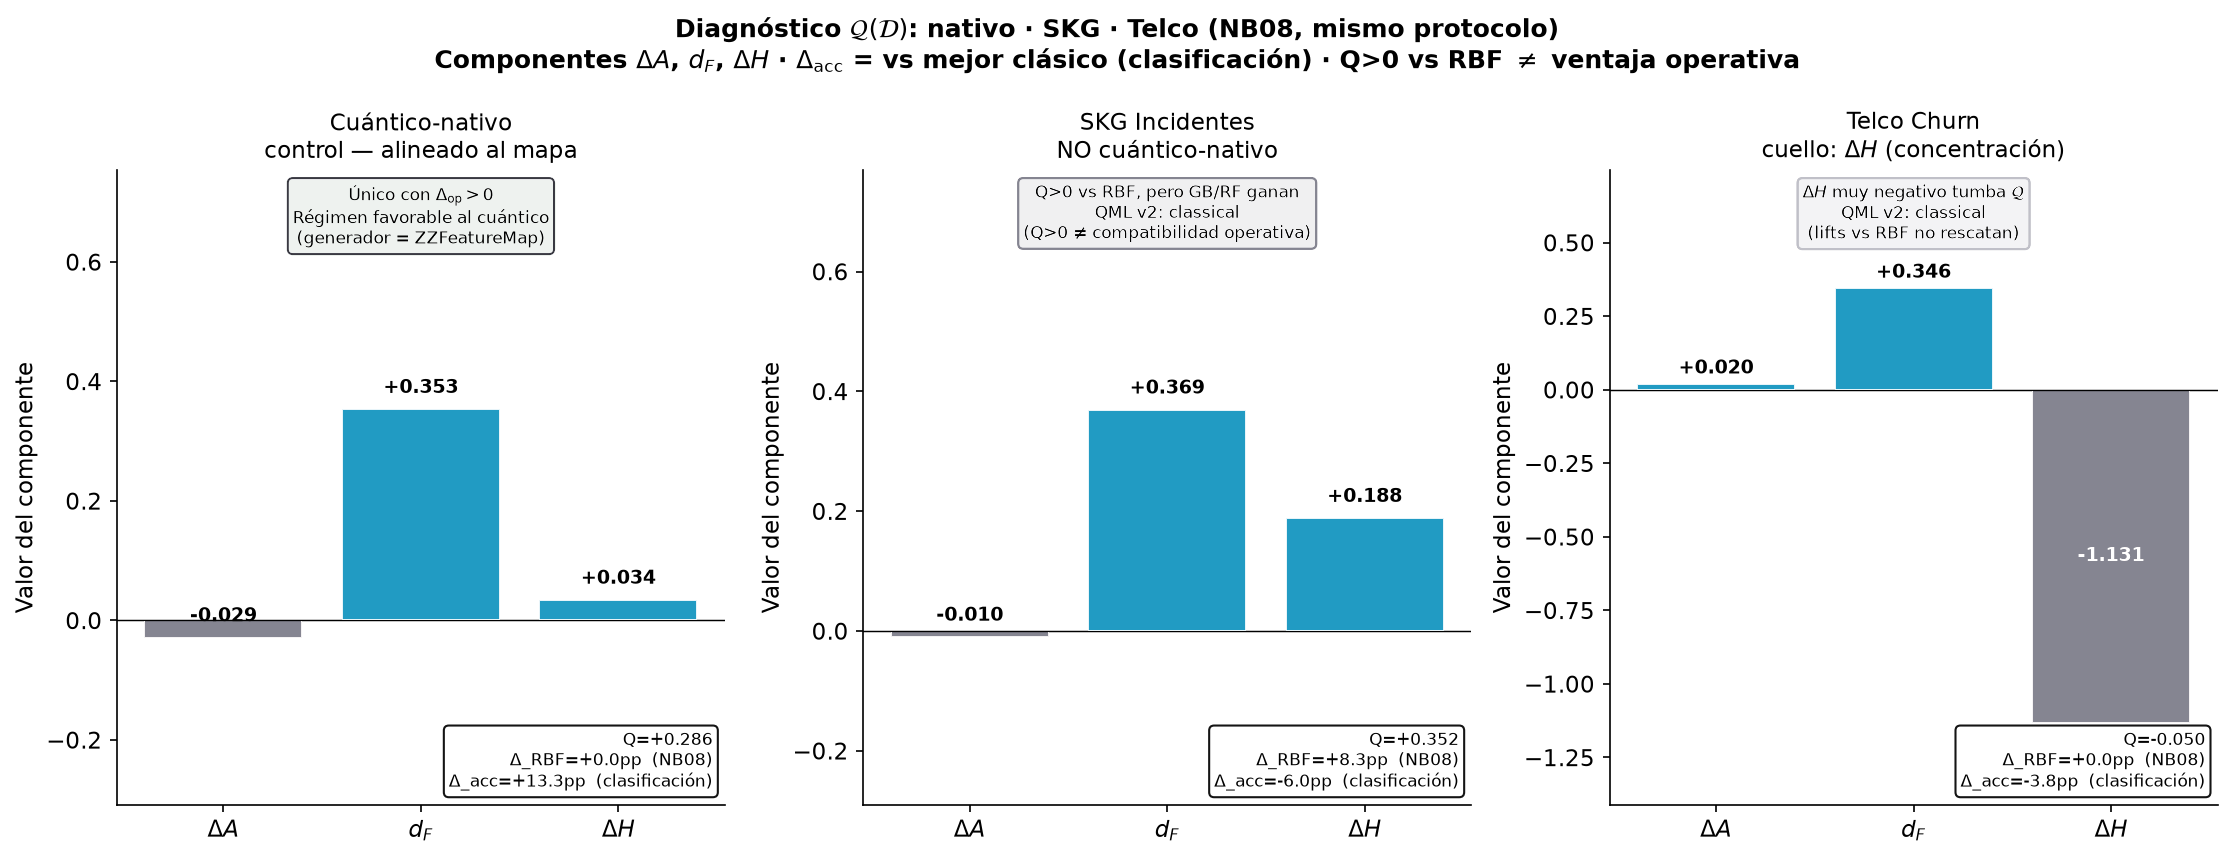
\includegraphics[width=\textwidth]{09_qcr_framework_diagnostico.png}
\end{column}
\begin{column}{0.48\textwidth}
\centering
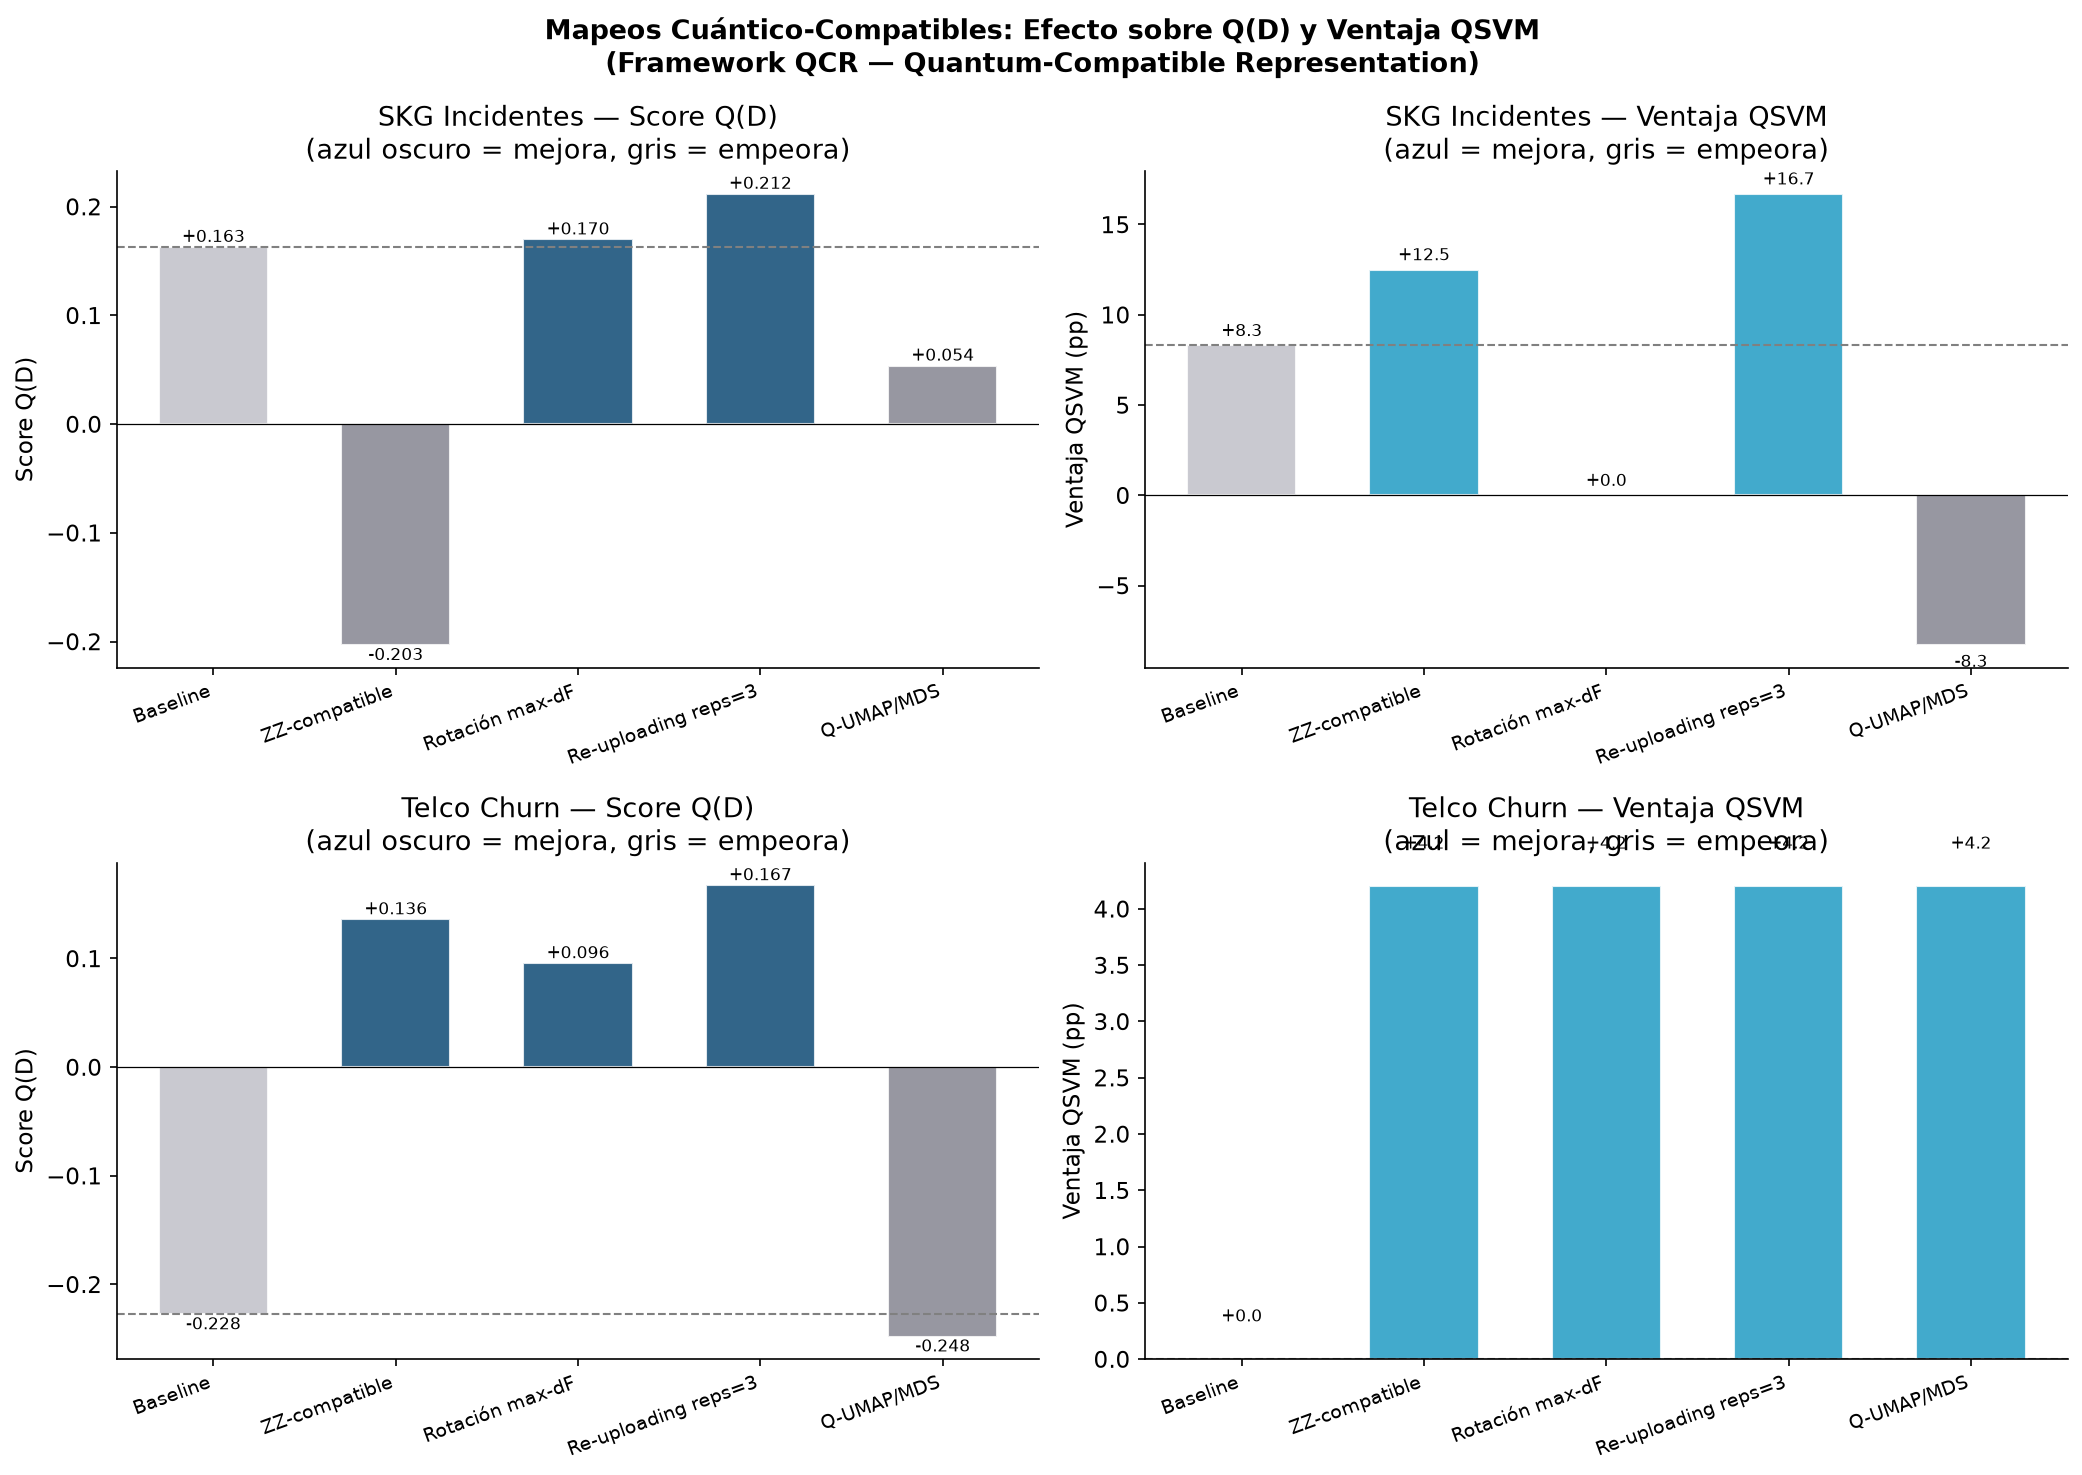
\includegraphics[width=\textwidth]{09_mapeos_comparativa.png}
\end{column}
\end{columns}
\vspace{0.3em}
\centering\footnotesize
Protocolo de diagnóstico $\to$ transformación candidata (rotación / re-uploading / \ldots).
Validación fuerte de QCR $=$ línea post-TFM.
\end{frame}

% =====================================================================
\section{Conclusiones}
% =====================================================================
\begin{frame}{Conclusiones}
\begin{enumerate}
  \item La ventaja cuántica en ciencia de datos es \textbf{real pero condicionada}.
  \item En kernels: alineación feature map $\leftrightarrow$ generador; ZZ es el mapa medido aquí.
  \item En optimización: QAOA/VQE aportan valor en QUBO de escala moderada (patrón híbrido).
  \item $\mathcal{Q}(\mathcal{D})$ es un diagnóstico útil \emph{a priori} ($\rho_S=0.833$ en barrido sintético).
  \item QCR queda \textbf{formalmente planteado}; no demostrado.
  \item Adopción recomendada: \textbf{selectiva e híbrida}, no sustitutiva del stack clásico.
\end{enumerate}
\end{frame}

\begin{frame}{Limitaciones (explicitadas)}
\begin{itemize}
  \item Simulación statevector (sin ruido NISQ de hardware).
  \item PCA a $n_q{=}2$ (~68\% de varianza descartada).
  \item Correlación $\mathcal{Q}$ en datos reales con $n$ pequeño (orientativa).
  \item QCR sin demostración fuerte.
  \item TSP: empate óptimo $\neq$ speedup.
\end{itemize}
\end{frame}

% =====================================================================
\section{Trabajo futuro}
% =====================================================================
\begin{frame}{Trabajo futuro}
\begin{columns}[T]
\begin{column}{0.48\textwidth}
\textbf{Corto plazo}
\begin{itemize}
  \item Hardware ruidoso / shots reales
  \item Más qubits, menos PCA
  \item Validación fuerte de QCR
\end{itemize}
\end{column}
\begin{column}{0.48\textwidth}
\textbf{Medio--largo plazo}
\begin{itemize}
  \item Benchmarks con separación formal
  \item Q-means / autoencoders
  \item Activación selectiva en pipelines productivos
\end{itemize}
\end{column}
\end{columns}
\end{frame}

\begin{frame}[plain]
\begin{center}
\vspace{1.8cm}
{\Large\bfseries Gracias}\\[0.6em]
{\large \textquestiondown{}Preguntas?}\\[1.6em]
{\small Juan David Prada Malagón \quad$\cdot$\quad UNIR}\\[0.4em]
{\footnotesize
\citep{preskill2018, biamonte2017, farhi2014, schuld2021, huang2021, liu2021, cerezo2021}}
\end{center}
\end{frame}

\begin{frame}[allowframebreaks]{Referencias (selección)}
\bibliographystyle{plainnat}
\begin{thebibliography}{99}
\bibitem[Biamonte et~al.(2017)]{biamonte2017}
Biamonte, J.\ et~al. (2017). \emph{Quantum machine learning}. Nature, 549, 195--202.

\bibitem[Cerezo et~al.(2021)]{cerezo2021}
Cerezo, M.\ et~al. (2021). \emph{Variational quantum algorithms}. Nat.\ Rev.\ Phys., 3, 625--644.

\bibitem[Farhi et~al.(2014)]{farhi2014}
Farhi, E., Goldstone, J., \& Gutmann, S. (2014). \emph{A quantum approximate optimization algorithm}. arXiv:1411.4028.

\bibitem[Fastovets et~al.(2019)]{fastovets2019}
Fastovets, D.\ et~al. (2019). \emph{Machine learning methods in quantum computing theory}. Proc.\ SPIE.

\bibitem[Huang et~al.(2021)]{huang2021}
Huang, H.-Y.\ et~al. (2021). \emph{Power of data in quantum machine learning}. Nat.\ Commun., 12, 2631.

\bibitem[Jordan \& Mitchell(2015)]{jordan2015}
Jordan, M.\ I., \& Mitchell, T.\ M. (2015). \emph{Machine learning: Trends, perspectives, and prospects}. Science, 349(6245), 255--260.

\bibitem[Liu et~al.(2021)]{liu2021}
Liu, Y., Arunachalam, S., \& Temme, K. (2021). \emph{A rigorous and robust quantum speed-up in supervised machine learning}. Nat.\ Phys., 17, 1013--1017.

\bibitem[Preskill(2018)]{preskill2018}
Preskill, J. (2018). \emph{Quantum computing in the NISQ era and beyond}. Quantum, 2, 79.

\bibitem[Schuld(2021)]{schuld2021}
Schuld, M. (2021). \emph{Supervised quantum machine learning models are kernel methods}. arXiv:2101.11020.

\bibitem[Thanasilp et~al.(2022)]{thanasilp2022}
Thanasilp, S.\ et~al. (2022). \emph{Exponential concentration and the limits of quantum ML}. arXiv:2208.11060.
\end{thebibliography}
\end{frame}

\end{document}
